\documentclass{article}

% packages
\usepackage[utf8]{inputenc}
\usepackage{pifont}
\usepackage{graphicx}
\graphicspath{{images/}}
\usepackage[hidelinks]{hyperref}
\usepackage{amsmath}
\usepackage{amssymb}
\usepackage{amsfonts}
\usepackage{mathtools}
\usepackage{xcolor}

\newcommand{\cmark}{\ding{51}}%
\newcommand{\xmark}{\ding{55}}%

% page format
\topmargin=-2cm
\textheight=23cm
\textwidth=19cm
\oddsidemargin=-1cm
\setlength{\parindent}{0pt}

\author{Guillaume W. Bres}
\title{Audio DSP}

\begin{document}

\maketitle

This project is an application of basic
signal processing on audio signal,
using Zynq/Zedboard platforms.

\tableofcontents

\newpage
\section{System}


\begin{center}
	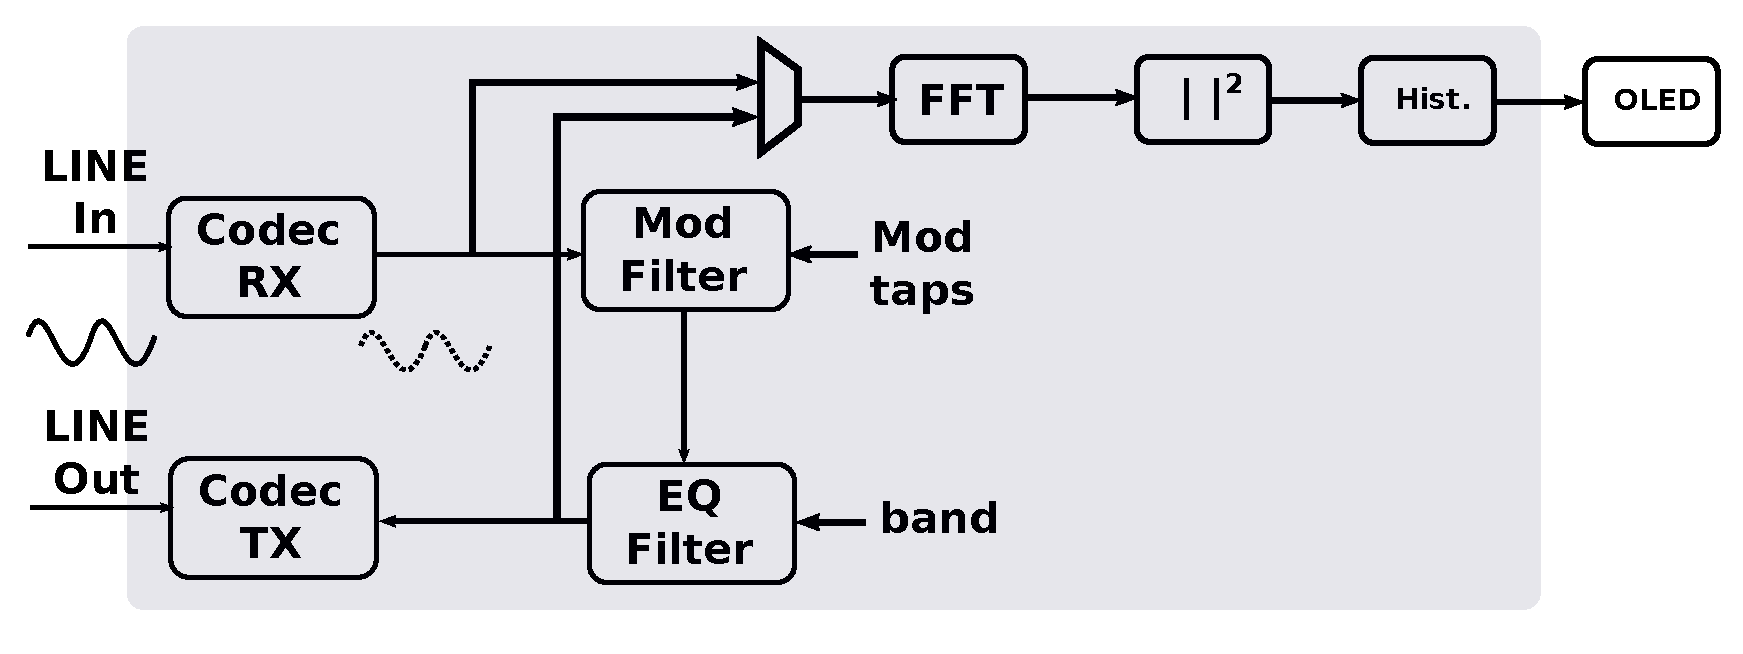
\includegraphics[width=0.75\linewidth]{bloc_design.pdf} \\
	Bloc design
\end{center}

All processing is real time and synchronous to the input
stream. The initial sample rate is 48 MHz, making the
input data rate 
which leads to a 1.152 Gb/s input data rate, this is much more than needed. \\

We reduce the internal sample rate to 24 kHz (a little more than needed),
reducing the bit rate to 576 kB/s.
Data rate reduction is done using a CIC decimation filter. \\

The modulation filter as well as the
EQ filter are controlled from the User Interface. \\

The FFT processes either the
direct RX input or the output signal.
This allows to visualize the effect
of the modulation \& the EQ filters.
Switching is done in real time on user specs. \\

The resulting power spectrum is converted to histogram
\& displayed on the onboard OLED display.
The display is 128x32 pixel wide, which in our case
gives a spectral resolution of 187.5 Hz
on the display, which is more than decent. \\

The internal data stream obviously needs a final
interpolation, this is done by a CIC interpolation
filter, feeding a 1.152 Gb/s stream to the TX side.
The CIC interpolation filter is strictly symmetrical
to the CIC decimation filter.

\newpage
\subsection{CIC filters}

CIC filter being defined by $R, M, N$ parameters where

\begin{itemize}
	\item R: decimation/interpolation factor
	\item M: time delay, can either be 1 or 2 cycle
	\item N: number of stages
\end{itemize}

\vspace{0.2cm}
To reduce the initial rate from 1.152 Gb/s we fix
$R = 128$. \\

Both the interpolation \& decimation filters
are comprised of a N stages of integration filters
\& comb filters. \\

The {\tt \$git/dsp/cic.py} Python script 
can plot the frequency response
of a given CIC filter:

\begin{verbatim}
   $git/dsp/cic.py R=4 M=1 N=12
   $git/dsp/cic.py R=8 M=2 N=4
\end{verbatim}

%\begin{center}
%	\includegraphics[width=0.75\linewidth]{cic_filters.pdf} \\
%  Switching from a decimation to an interpolation is simply
%  changing the internal ordering and obviously performing
%  either a decimation or an interpolation in between
%  comb/integration stages.
%\end{center}

\begin{itemize}
	\item an integrator stage is defined as $H(z) = \frac{1}{1 - z^{-1}}$\\
	
	\item a comb stage is defined as $H(z) = 1 - z^{-M}$\\
	
	\item total CIC filter response is therefore $H(z) = \left| \frac{1 - z^-M}{1 - z^{-1}} \right|^N$
	
	\item the total magnitude response is approximated by
	$H(\nu) = \left| \frac{\sin(R M \pi \nu)}{R M \sin(\pi \nu)} \right|^N$

	\item the worst alias is encountered at frequency $\nu = \frac{3}{2MR}$

	\item the total filter gain is $(RM)^N$
	\item hence the total bit growth in our implementation
	will be $\left[ log_2\left(RM^N\right) \right]_\text{ceil}$
\end{itemize}

\newpage
Increasing N (number of stages) increases the filter performance:

\begin{center}
	\begin{minipage}{0.49\linewidth}
		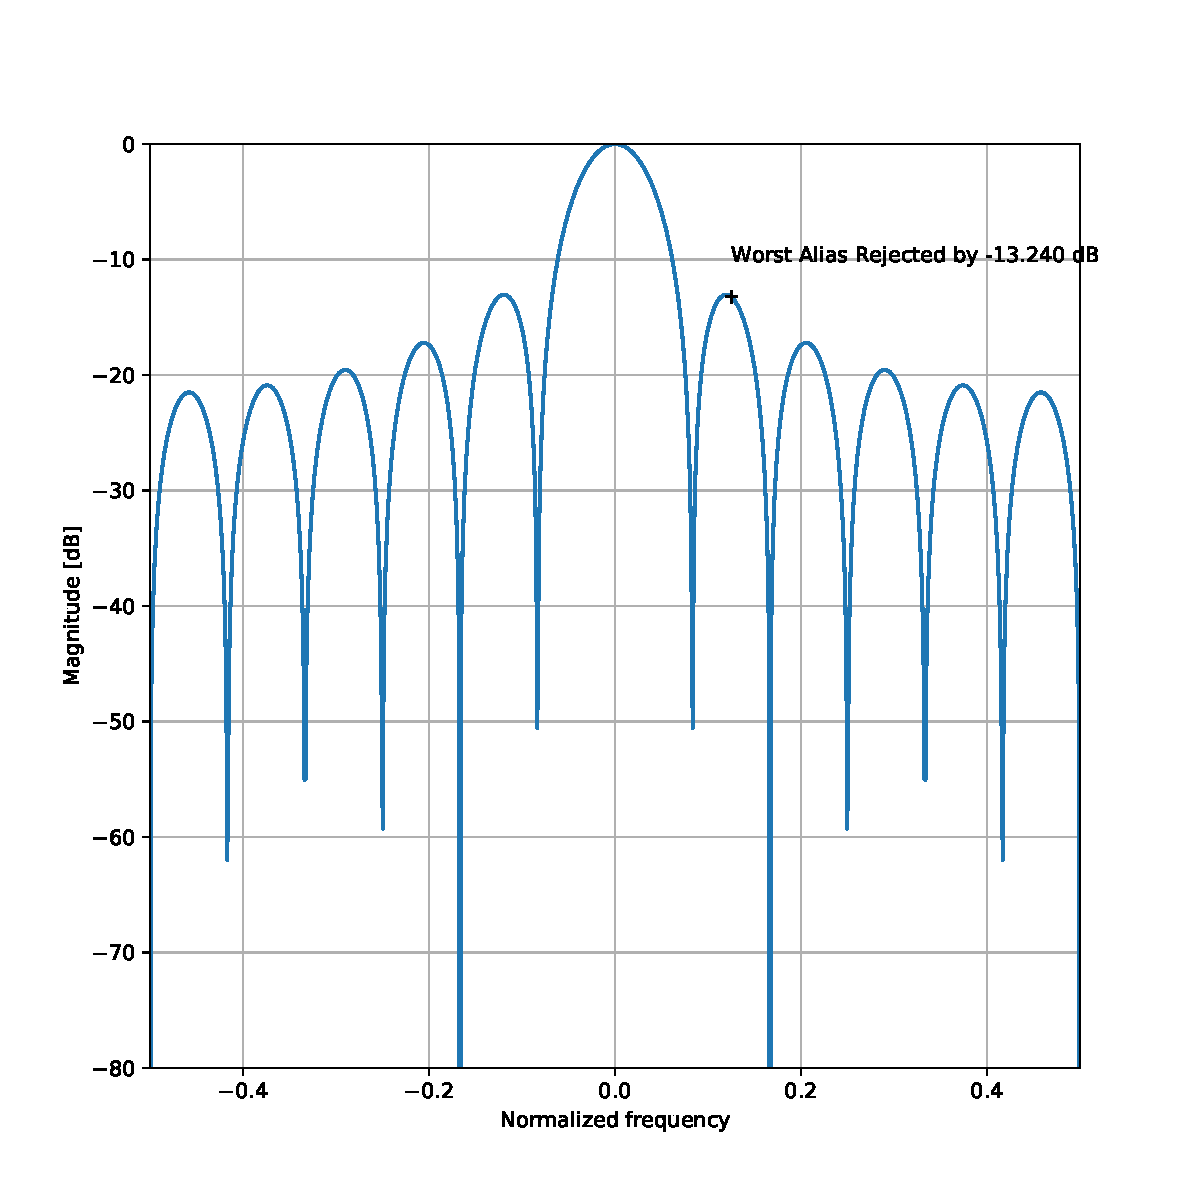
\includegraphics[width=0.99\linewidth]{cic_r12_n2.pdf} \\
		Comparing a CIC decimation filter with N=2 stages,
		the worst alias is rejected by -13 dB
	\end{minipage}
	\begin{minipage}{0.49\linewidth}
		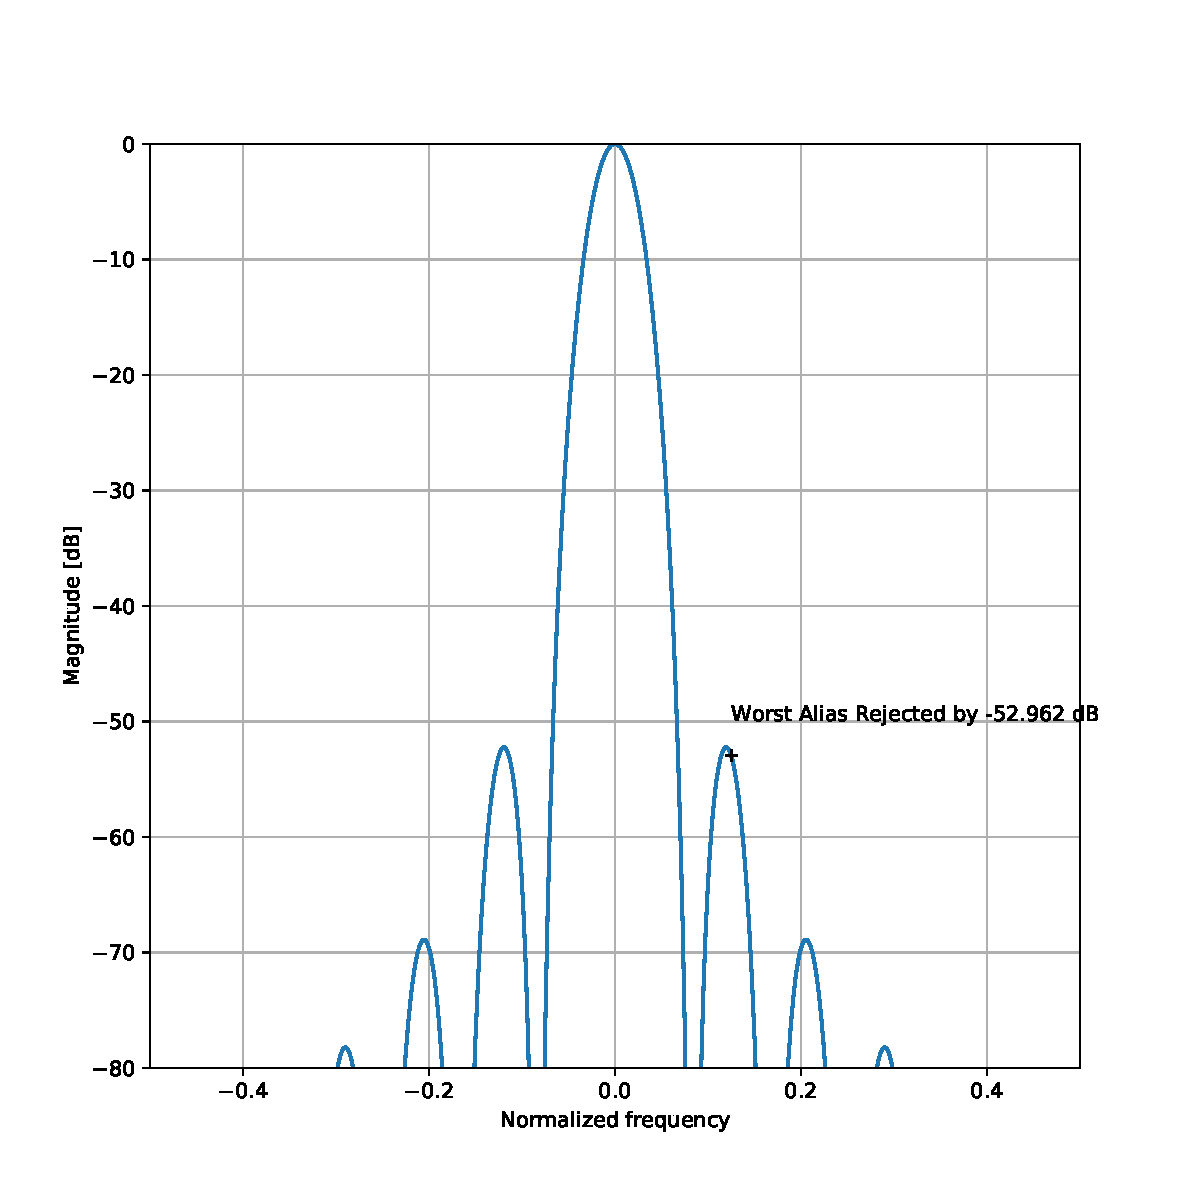
\includegraphics[width=0.99\linewidth]{cic_r12_n8.pdf} \\
		Increasing the number of stages to N=8
		improves the worst alias rejection to -53 dB
	\end{minipage}
\end{center}

We fix $N=8$ in our case, not to consume too much ressources.
This will give a rejection of
-53 dB for the worst alias ever encountered. \\

As you can see, the CIC filter frequency reponse has a
$f(\nu) = \frac{sin(\nu)}{\nu}$ shape.
Which means we completely lose the flatness of within
the system bandwidth, and the transition bandwidth to cutoff
is very large. \\

To compensate for the flatness loss and to reduce
the transition bandwidth, 
we introduce a compensation filter (in the form of an FIR
filter) after the CIC decimation filter
and prior the CIC interpolation filter.

\subsection{CIC compensation filter}

The compensation filter response is the exact inverse
of the CIC filter response $G(\nu) = \frac{1}{H(\nu)}$ 
within the new established band, ranging
from 0 to $\frac{f_s}{R}$,
$\frac{f_s}{R}$ being the first null of the $\frac{sin(\nu)}{\nu}$ response. \\

The CIC compensation filter is designed
using the python script {\tt \$git/dsp/cic-compensator.py}. 

\begin{verbatim}
   $git/dsp/cic-compensator.py R=4 N=12 BW=30
   $git/dsp/cic-compensator.py R=8 N=4 BW=45 ncoef=128
\end{verbatim}

Use BW (in \%) to set the pass band edge
location within the new established Nyquist band.
The ncoef parameter allows to compare different
implementation of the FIR filter.

\begin{center}
	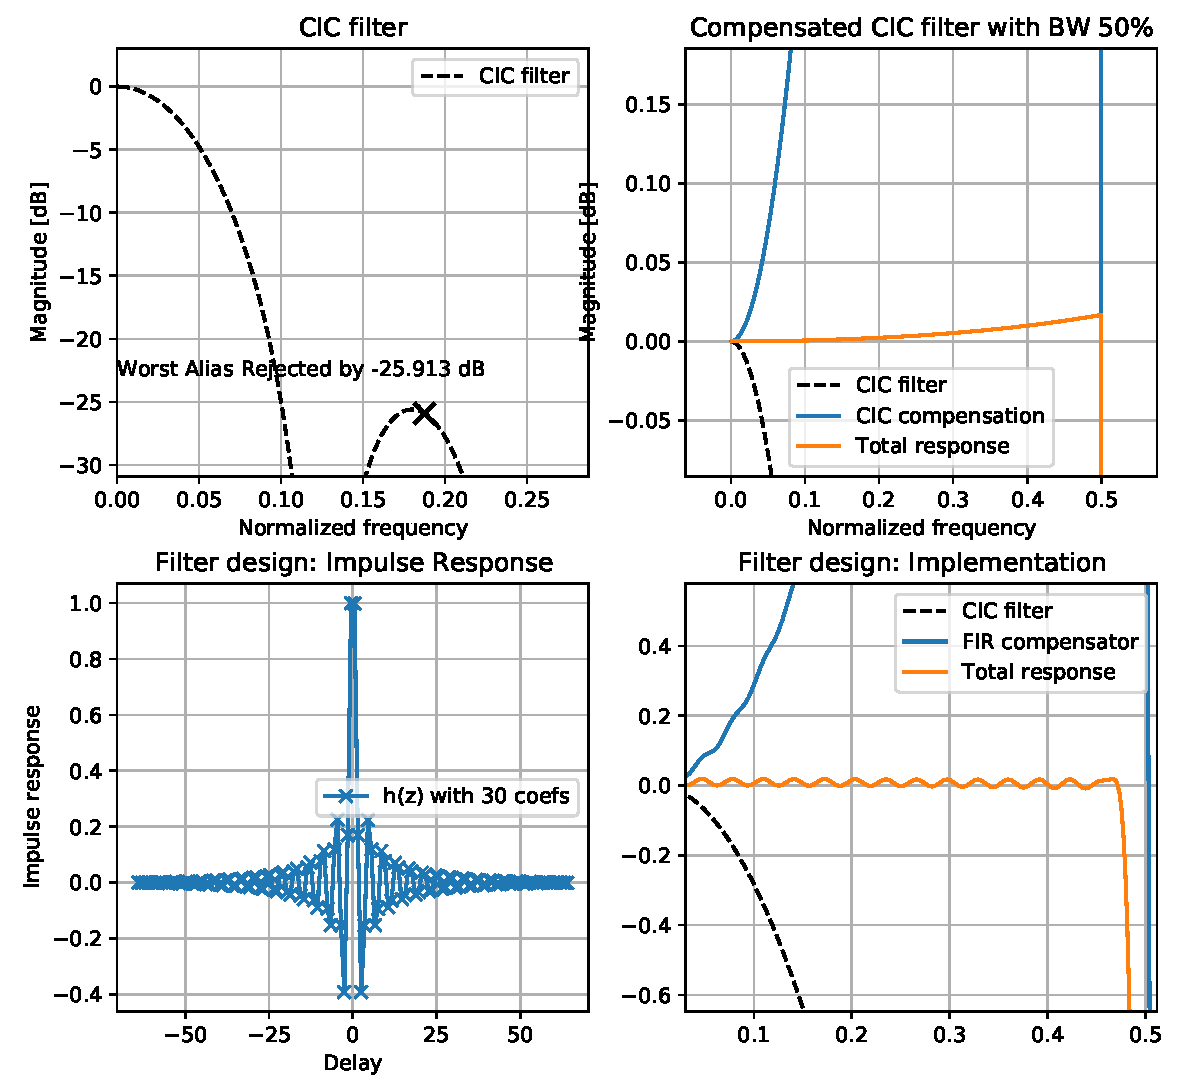
\includegraphics[width=0.75\linewidth]{fir-des-2.pdf} \\
	The CIC filter compensator designer designs a CIC
	filter to compensate for the CIC filtering stage.
	One can compare the effect of the BW cut off frequency
	(design the new user bandwidth) and the ripple effect,
	for different FIR filters implementation.
\end{center}

Upper left: theoretical CIC filter as described in previous
section. \\

Upper right: theoretical CIC filter versus its optimum
compensation, for a given BW parameter.
Total theoretical response is CIC+FIR. \\

Below - left: designed Impulse Response to be implemented,
for given BW and ncoef parameters. \\

Below - right: filter implementation: theoretical
CIC filter compensated by implemented FIR filter.
Total implemented response is CIC+FIR. \\

CIC filter compensation 
will be implemented in both the decimation
\& the interpolation filter, using
Xilinx's optimized FIR filter IP core. \\

The CIC decimation is very important
to our system, without heavily downsampling
the input signal (we chose R=128),
the displayed FFT resolution would be
37.5 MHz, which is totaly unusable for audio data.
The Modulation Filter \& EQ filter would require so 
many bands to be computated that it would also be impossible
to implement them in the system.

\subsubsection{CIC interpolation filter}

Using previously designed compensated CIC decimator,
we reduce the input rate by a factor of 128.
We need to interpolate by a factor of 128 prior
outputing the signal to the DAC.


\newpage
\subsection{Equalization filter}

The EQ filter allows the user 
to modify the signal's frequency response,
in real time. \\

The frequency response is divided into 16 bands,
considering our internal sample rate of 
$f_s = \frac{48e8}{128} = 24$ kHz,
each band is 1.5 kHz wide. \\

The user interface allows the user
to define the weighting of each band,
so define the custom frequency response
$H(\nu)$. \\

The GUI transforms $H(\nu)$ into $h(z)$
to be applied in the FIR filter:

\begin{equation}
	\begin{split}
	h(z) = FFT^{-1}\left(H(z)\right) = Bilienear(H(\nu))
	\end{split}
\end{equation}

\newpage
\subsection{FFT Histogram}

The Histogram IP core converts
the power spectrum from the
magnitude IP core
to a histogram to be displayed on the OLED. \\

It is a simple mapping of the resulting
power spectrum to a 2D array (X,Y) describing
the power spectrum along a frequency axis. \\ 

%\begin{center}
%	\includegraphics[width=0.75\linewidth]{fft_histogram.pdf} \\
%\end{center}

\section{Simulation}

\subsection{GHDL}

Most IPs are simple unitary functions
and can be simulated using {\tt ghdl}.
Any IP that comes with a {\tt /sim/Makefile}
can be simulated with {\tt ghdl}.

Install {\tt ghdl} to easily
simulate modules that come with a testbench:

\begin{verbatim}
git clone https://github.com/ghdl/ghdl
cd ghdl
./configure
make
sudo make install
\end{verbatim}

Once this is done, you can safely simulate a module
that comes with a testbench by using {\it make}
in its {\tt sim} folder.
For example:

\begin{verbatim}
cd $git/ip/adau1761/sim
make
\end{verbatim}

\subsection{Vivado - {\tt xsim}}

IPs that require Xilinx's dedicated functions,
such as BRAM or FIFOs to buffer the input/output
data, can only be simulated in Vivado.

To simulate those IPs on your side, either
import the IP sources \& dependencies and the testbench
into Vivado, or use the {\tt sim-project.tcl} if
it is delivered with the IP.

\end{document}
